%
% 1-problem.tex
%
% (c) 2023 Prof Dr Andreas Müller
%
\section{Problemstellung
\label{buch:variation:section:problemstellung}}
\kopfrechts{Problemstellung}
Das Brachistochronenproblem, welches Johann Bernoulli im Jahr 1696
gestellt hat, war nicht das erste Optimierungsproblem für eine 
gesuchte Funktion, welches Physiker betrachtet haben.
Aber es darf als Ausgangspunkt für die Entwicklung der Variationsrechnung
betrachtet werden.
Alle diese Probleme zeichnen sich dadurch aus, dass Extremwerte
einer Grösse, die von allen Werten einer unbekannten Funktion abhängt,
gefunden werden sollen.
Die von Euler und Lagrange entwickelte Theorie zeigt, dass eine
Lösung für diese globale Eigenschaft immer auf eine lokale Bedingungen,
genauer auf eine Differentialgleichung reduziert werden kann, für deren
Lösung bereits eine ausgefeilte Theorie existiert.

%
% Der Anfang: das Brachistochronenproblem von Bernoulli
%
\subsection{Der Anfang: Das Brachistochronenproblem von Bernoulli
\label{buch:variation:problem:subsection:brachistochrone}}
%%
% brachistochronenproblem.tex -- Brachistochronenproblem
%
% (c) 2021 Prof Dr Andreas Müller, OST Ostschweizer Fachhochschule
%
\documentclass[tikz]{standalone}
\usepackage{amsmath}
\usepackage{times}
\usepackage{txfonts}
\usepackage{pgfplots}
\usepackage{csvsimple}
\usetikzlibrary{arrows,intersections,math}
\begin{document}
\def\skala{1}
\def\r{1.5}
\pgfmathparse{3.14159/180}
\xdef\m{\pgfmathresult}
\def\xwert#1{\r*((#1)*\m-sin(#1))}
\def\ywert#1{\r*(cos(#1)-1)}
\def\punkt#1{ ({\r*((#1)*\m-sin(#1))},{\r*(cos(#1)-1)}) }
\begin{tikzpicture}[>=latex,thick,scale=\skala]

\draw[color=gray!50] plot[domain=0:360,samples=360]
	({\r*((\x)*\m-sin(\x))},{\r*(cos(\x)-1)});

\draw[->] (-0.1,0) -- (10,0) coordinate[label={$x$}];
\draw[->] (0,0.1) -- (0,-3.5) coordinate[label={left:$y$}];

\draw ({\m*\r*180},0.05) -- ({\m*\r*180},-0.05);
\node at ({\m*\r*180},0) [above] {$\frac{\pi}2\mathstrut$};
\draw ({\m*\r*360},0.05) -- ({\m*\r*360},-0.05);
\node at ({\m*\r*360},0) [above] {$\pi\mathstrut$};

\draw[line width=0.2pt]  ({\xwert{60}},0) -- \punkt{60};
\node at ({\xwert{60}},0) [above] {$a\mathstrut$};
\draw ({\xwert{60}},0.05) -- ({\xwert{60}},-0.05);

\draw[line width=0.2pt]  ({\xwert{160}},0) -- \punkt{160};
\node at ({\xwert{160}},0) [above] {$b\mathstrut$};
\draw ({\xwert{160}},0.05) -- ({\xwert{160}},-0.05);

\draw[color=red,line width=1.2pt] plot[domain=60:160,samples=100]
	({\r*((\x)*\m-sin(\x))},{\r*(cos(\x)-1)});

\fill[color=red] \punkt{60} circle[radius=0.08];
\node at \punkt{60} [above right] {$A$};
\fill[color=red] \punkt{160} circle[radius=0.08];
\node at \punkt{160} [below] {$B$};
\fill[color=red] \punkt{100} circle[radius=0.08];
\node at \punkt{100} [below left] {$M$};

\end{tikzpicture}
\end{document}


%
% bernoulli.tex -- Problem von Bernoulli
%
% (c) 2021 Prof Dr Andreas Müller, OST Ostschweizer Fachhochschule
%
\documentclass[tikz]{standalone}
\usepackage{amsmath}
\usepackage{times}
\usepackage{txfonts}
\usepackage{pgfplots}
\usepackage{csvsimple}
\usetikzlibrary{arrows,intersections,math}
\definecolor{darkred}{rgb}{0.8,0,0}
\begin{document}
\def\skala{1}
\def\r{2}
\def\m{4}
\begin{tikzpicture}[>=latex,thick,scale=\skala,
declare function = {
	X(\t) = \r*(-sin(180*\t/3.14159)+\t);
	Y(\t) = -\r*(1-cos(180*\t/3.14159));
	etaX(\t,\a) = 0;
	etaY(\t,\a) = 0.015*\a*(X(\t)*(X(\m)-X(\t));
}]

\coordinate (A) at (0,0);
\coordinate (B) at ({X(\m)},{Y(\m)});
\coordinate (M) at ({X(0.7*\m)},{Y(0.7*\m)});

\foreach \a in {-4,-3,...,7}{
	\draw[color=gray!40,line width=1.0pt] plot[domain=0:\m,samples=40]
		({X(\x)+etaX(\x,\a)},{Y(\x)+etaY(\x,\a)});
}

\draw[color=darkred,line width=1.4pt]
	plot[domain=0:\m,samples=40] ({X(\x)},{Y(\x)});

\draw[->] (-0.1,0) -- ({X(\m)+0.5},0) coordinate[label={$x$}];
\draw[->] (0,0.1) -- (0,{-2*\r-1.4}) coordinate[label={left:$y$}];

\fill[color=darkred] (A) circle[radius=0.08];
\fill[color=darkred] (B) circle[radius=0.08];
\fill[color=darkred] (M) circle[radius=0.08];
\node[color=darkred] at (A) [above] {$A$};
\node[color=darkred] at (B) [right] {$B$};
\node[color=darkred] at (M) [above right] {$M$};

\end{tikzpicture}
\end{document}


Im Jahr 1696 publiziert der Basler Mathematiker Johann Bernoulli, damals
Professor für Mathematik in Groningen das folgende Problem in der
von Leibniz herausgegebenen Zeitschrift {\em Acta eruditorum}:
\begin{center}
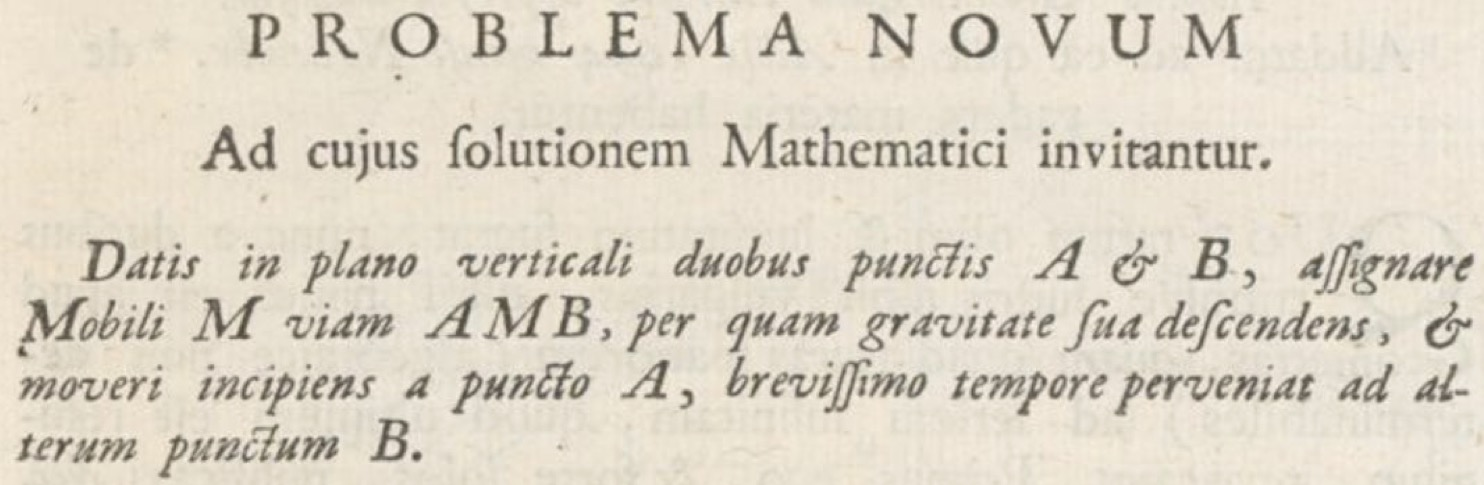
\includegraphics[width=0.8\textwidth]{chapters/020-variation/images/latein.jpg}
\end{center}
Zu deutsch:
\begin{quote}
Neue Aufgabe, zu deren Lösung die Mathematiker eingeladen werden.
Gegeben zwei Punkte $A$ und $B$ in einer vertikalen Ebene, finde
die Bahn $AMB$ eines Punktes $M$, der unter der Wirkung seines
Gewichtes in kürzester Zeit vom Punkt $A$ zum anderen Punkt $B$ absteigt.
\end{quote}
Die Situation der Aufgabenstellung ist in
Abbildung~\ref{buch:variation:problem:fig:bernoulli}
dargestellt.
Bernoulli hat als Lösung gefunden, dass die Kurve eine Ausschnitt
aus einer Zykloide (in der Abbildung grau) sein muss.
Seine Lösung beruhte auf der Beobachtung, dass sich das Problem analog
zu einem Lichtausbreitungsproblem ist, für welches Fermat bereits
eine Lösung gefunden hat.
Den Zusammenhang zwischen dem Brachistochronenproblem und der geometrischen
Optik wird in \cite{buch:broer} ausführlich beschrieben.

Das Koordinatensystem wählen wir so, dass der Nullpunkt mit $A$ zusammenfällt
und die $y$-Achse in Richtung der Schwerkraft zeigt.
Da die Reibung vernachlässigt wird, ist die Energie des Massepunktes
erhalten.
Sie setzt sich aus der potenziellen und der kinetischen Energie
zusammen.
Die potenzielle Energie ist $-mgy$, die kinetische Energie ist
$\frac12mv^2$.
Zu Beginn ist die Gesamtenergie 0.
Die Energieerhaltung wird daher zu
\[
0=\frac12mv^2-mgy
\quad\Rightarrow\quad
\frac12mv^2=mgy
\quad\Rightarrow\quad
v^2=2gy
\quad\Rightarrow\quad
v(y)
=
\sqrt{2g}\!\sqrt{y}
=
\!\sqrt{2gy}.
\]
Durch Wahl einer anderen Zeiteinheit kann die Gleichung noch weiter
vereinfacht zu
\(
v(y) = \sqrt{y}
\)
vereinfacht werden.
Gesucht ist also die zeitlich kürzeste Bahn eines Teilchens, 
dessen Geschwindigkeit auf bekannte Art $v(y)$ von der vertikalen
Koordinate abhängt.

%
% Das Fermat-Problem
%
\subsection{Das Fermat-Prinzip}
Bereits Fermat hat erkannt, dass das Brechnungsgesetz von Snellius
als Lösung eines Extremalproblems verstanden werden kann.

\begin{satz}[Fermat-Prinzip]
\label{buch:variation:problem:satz:fermat-prinzip}
Licht breitet sich immer entlang des Weges aus, der die geringste
Zeit braucht.
\end{satz}

Die Geschwindigkeit des Lichts in einem Medium hängt vom Medium ab.
Die Vakuumlichtgeschwindigkeit $c$ kann von der Ausbreitungsgeschwindigkeit
in einem Medium nicht übertroffen werden, die Ausbreitungsgeschwindigkeit
in einem Medium kann daher immer als $c/n$ geschrieben werden, wobei
$n\ge 1$ der sogenannte {\em Brechungsindex} oder die {\em optische Dichte}
des Mediums ist.
\index{Brechungsindex}%
\index{Dichte, optische}%
\index{optische Dichte}%
Der Brechungsindex in einem Medium hängt ausserdem von der Wellenlänge ab.
verschiedenfarbiges Licht wird daher mehr oder weniger stark gebrochen,
Was in Prismen zur Aufspaltung des Lichts in ein Spektrum verwendet
werden kann, aber in einem optischen System auch zu Farbrändern an
hellen Objekten führen kann.
Aus dem Fermatprinzip ergibt sich jetzt das Brechungsgesetz von 
Snellius.

\begin{satz}[Snellius]
\label{buch:variation:problem:satz:snellius}
Sei $c/n_i$ die Geschwindigkeit, mit der sich Licht im Medium $M_i$
ausbreitet.
Ein Lichtstrahl von $A_1$ nach $A_2$ geht durch denjenigen Punkt $B$ 
auf der Grenzfläche zwischen den Medien, für den sich die Sinus der
Winkel $\alpha_i$ zwischen den Strahlen und der Normalen zur Grenzfläche
umgekehrt wie die $n_i$ verhalten, wenn also das Brechungsgesetz
\[
\frac{\sin\alpha_1}{\sin\alpha_2}
=
\frac{n_2}{n_1}
\]
gilt.
\end{satz}

%
% snellius.tex
%
% (c) 2024 Prof Dr Andreas Müller
%
\begin{figure}
\centering
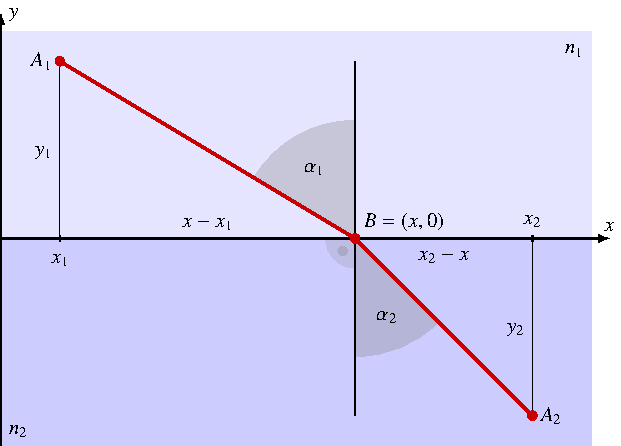
\includegraphics{chapters/020-variation/images/snellius.pdf}
\caption{Herleitung des Brechnungsgesetzes von Snellius aus dem
Fermat-Prinzip (Beweis von Satz~\ref{buch:variation:problem:satz:snellius}).
\label{buch:variation:problem:fig:snellius}}
\end{figure}


\begin{proof}
Ohne der Beschränkung der Allgmeinheit können wir auf die Betrachtung
einer Ebene beschränken, die die beiden Punkte $A_i$ enthält und senkrecht
auf der Grenzfläche steht (Abbildung~\ref{buch:variation:problem:fig:snellius}).
Wir dürfen weiter annehmen, dass die $x$-Achse in der Grenzfläche liegt 
und die Punkte $A_i$ die Koordinaten $(x_i,y_i)$ und der Punkt $B$ die
Koordinaten $(x,0)$ hat.
Es ist derjenige Punkt $x$ zu bestimmen, für den die Lichtzeit entlang 
des Pfades $A_1BA_2$ minimal wird.
Diese Zeit ist
\begin{align*}
t
&=
\frac{\overline{A_1B}}{c/n_1}
+
\frac{\overline{BA_2}}{c/n_2}
\\
ct
&=
n_1\overline{A_1B}
+
n_2\overline{A_2B}
\\
&=
n_1\!\sqrt{(x-x_1)^2 + y_1^2}
+
n_2\!\sqrt{(x_2-x)^2 + y_2^2}
\end{align*}
Das Minimum wird bei einer Nullstelle der Ableitung nach $x$ gefunden,
also bei einer Lösung der Gleichung
\begin{align*}
0
&=
n_1\frac{2(x_1-x)x}{\sqrt{(x_1-x)^2+y_1^2}}
+
n_2\frac{-2(x-x_2)x}{\sqrt{(x_2-x)^2+y_2^2}}.
\intertext{Indem man den zweiten Term auf der rechten Seite auf die linke
Seite bringt und durch $x$ dividiert, erhält man}
n_1
\frac{x_1-x}{\sqrt{(x_1-x)^2+y_1^2}}
&=
n_2
\frac{x-x_2}{\sqrt{(x_2-x)^2+y_2^2}}.
\end{align*}
Der Nenner ist auf beiden Seiten die Hypothenuse eines rechtwinkligen
Dreiecks, welches als Ankathete die Normale zur Grenzfläche hat.
Der Zähler ist die Gegenkathete des Winkels $\alpha_i$ zwischen der
Hypothenuse und der Normalen.
Daher ist der Quotient der Sinus des Winkels oder
\begin{equation}
n_1 \sin\alpha_1 = n_2 \sin\alpha_2.
\label{buch:variation:problem:eqn:snelliusinvariante}
\end{equation}
Die Gleichung~\eqref{buch:variation:problem:eqn:snelliusinvariante}
ist gleichbedeutend mit dem Brechungsgesetz
\[
\frac{\sin\alpha_1}{\sin\alpha_2}
=
\frac{n_2}{n_1}
\]
von Snellius.
\end{proof}

Das Prinzip von Fermat etabliert das Brechungsgsetz also Lösung eines
Extremalproblems.
Die Natur wählt für einen Lichtstrahl den zeitlich kürzesten Weg.
Der Beweis des Satzes von Fermat zeigt, dass entlang des Lichtstrahls
an jeder Grenzfläche zwischen Medien die Bedingung
\eqref{buch:variation:problem:eqn:snelliusinvariante}
erfüllt.
Dies gilt auch, wenn der Strahl durch mehrere Schichten mit
unterschiedlichem Brechungsindex dringt.
In jeder Schicht hat das Produkt $n\sin\alpha$ den gleichen Wert.

Wenn die optische Dichte $n$ eine Funktion von $n(y)$ ist, dann
wird der Lichtstrahl nicht nur in diskreten Punkten geknickt, sondern
entlang des ganzen Strahles gekrümmt.
In jedem Punkt des Strahls muss aber weiterhin $n(y)\sin\alpha(y)$
gelten, wobei $\alpha(y)$ der Winkel zwischen der Vertikalen und
der Tangente an den Strahl ist.

Folgt der Strahl der Kurve $x(y)$, die mit der vertikalen den Winkel
$x'(y) = \tan\alpha(y)$ einschliesst, dann lässt sich der Sinus
auch durch die Ableitung als
\[
\sin\alpha(y)
=
\frac{x'(y)}{\pm\!\sqrt{x'(y)^2+1}}
\]
ausdrücken.
Aus der Form~\eqref{buch:variation:problem:eqn:snelliusinvariante}
des Brechungsgesetztes wird dann die Gleichung
\begin{equation}
n_1\sin\alpha(y)
=
\frac{n_1(y)x'(y)}{\pm\!\sqrt{x'(y)^2+1}}
=
\operatorname{const}
\qquad\Rightarrow\qquad
\frac{n_1(y)^2x'(y)^2}{x'(y)^2+1}=C.
\label{buch:variation:eqn:fermatdgl}
\end{equation}
Dies ist eine Differentialgleichung für die Funktion $x(y)$.
Sie kann auch in die Form
\[
x'(y)^2
=
\frac{C}{(n_1(y)^2-C)}
\]
gebracht werden.

%
% Das Brachistochronenproblem als Lichtausbreitungsproblem
%
\subsubsection{Das Brachistochronenproblem als Lichtausbreitungsproblem}
Das Fermat-Prinzip besagt, dass ein Lichtstrahl, der sich in einem Medium
mit der Geschwindigkeit $c/n(y)$ ausbreitet, die Gleichung 
\eqref{buch:variation:eqn:fermatdgl} erfüllt.
Beim Brachistochronenproblem ist die Geschwindigkeit $v(y)=\!\sqrt{y}$ und 
damit $n(y) = c/\!\sqrt{y}$.
Eine Brachistochrone ist also eine Kurve, die die aus
\eqref{buch:variation:eqn:fermatdgl} folgende Gleichung
\begin{equation}
\frac{(c^2/y) x'(x)^2}{(1+x'(y)^2}
=
C
\qquad\Rightarrow\qquad
\frac{x'(y)^2}{(1+x'(y)^2)y}
=
K
\label{buch:variation:problem:eqn:bernoullidgl}
\end{equation}
erfüllen.
Es genügt somit, eine Lösung dieser Differentialgleichung zu finden,
die durch die beiden Punkte $A$ und $B$ geht.
Allerdings ist die Lösung der Differentialgleichung
\eqref{buch:variation:problem:eqn:bernoullidgl}
nicht offensichtlich, sie wird im nächsten Abschnitt diskutiert.

Bernoullis Weg zu einer Lösung des Brachistochronenproblems bestand
also vor allem in der Erkenntnis, dass das Brachistochronenproblem mit
Hilfe einer Analogie zur Lichtausbreitung auf die Lösung einer
Differentialgleichung reduzieren lässt.
Die globale Bedingung, dass die benötigte Zeit minimiert werden muss,
konnte durch eine lokale Bedingung an die Steigung der Kurve ersetzt
werden.

%
% Die Bernoullische Lösung
%
\subsubsection{Die Bernoullische Lösung}
Bernoulli hat gefunden, dass die Brachistochrone ein Zykloidenbogen ist.
Dies ist auch der Tatsache geschuldet, dass den Mathematikern seiner
Zeit die Eigenschaften vieler ebener Kurven so gut bekannt waren, dass
sie die richtige Lösung aus der Differentialgleichung mehr oder weniger
hätten erraten können.
In der heutigen Zeit werden diese Kurven oft eher als Kuriositäten
im Unterricht behandelt und bald wieder vergessen.

Die direkte Lösung der Differentialgleichung
\eqref{buch:variation:problem:eqn:bernoullidgl}
ist nicht ganz einfach.
Statt sie hier durchzuführen, verweisen wir auf
Abschnitt~\ref{buch:variation:eulerlagrange:subsection:brachistochrone},
in dem das Brachistochronenproblem mit Hilfe der allgemeinen
Theorie und der Euler-Lagrange-Differentialgleichung gelöst wird.

Auch wenn wir die Lösung nicht direkt aus der Differentialgleichung
bestimmen wollen, können wir immerhin verifizieren, dass die Zykloide
eine Lösung der Gleichung~\eqref{buch:variation:problem:eqn:bernoullidgl}
ist.
Wir verwenden dazu die Parameterdarstellung einer Zykloide und
setzten sie in die Gleichung~\eqref{buch:variation:problem:eqn:bernoullidgl}
ein.
Die Zykloide hat die Parametrisierung
\[
\left.
\begin{aligned}
x &= r(\varphi - \sin\varphi) 
\\
y &= r(1-\cos\varphi)
\end{aligned}
\right\}
\quad
\text{mit der Ableitung}
\quad
\left\{
\begin{aligned}
\dot{x}(\varphi) &= r(1-\cos\varphi)\\
\dot{y}(\varphi) &= r\sin\varphi
\end{aligned}
\right.
\]
für $\varphi\in\mathbb{R}$, wie man aus der
%
% zykloide.tex
%
% (c) 2024 Prof Dr Andreas Müller
%
\begin{figure}
\centering
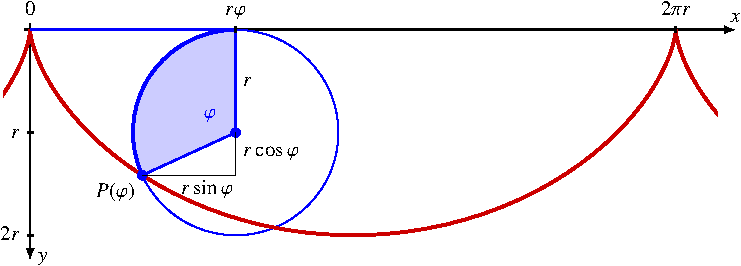
\includegraphics{chapters/020-variation/images/zykloide.pdf}
\caption{Parametrisierung der Zykloide, die durch Abrollen eines
Kreises mit Radius $r$ auf der $x$-Achse entsteht.
Für $t=0$ berührt der Kreis die $x$-Achse im Nullpunkte.
\label{buch:variation:problem:fig:zykloide}}
\end{figure}

Abbildung~\ref{buch:variation:problem:fig:zykloide} ablesen kann.
Die Ableitung ist
\[
x'(y)
=
\frac{\dot{x}(\varphi)}{\dot{y}(\varphi)}
=
\frac{1-\cos\varphi}{\sin\varphi}.
\]
Eingesetzt in \eqref{buch:variation:problem:eqn:bernoullidgl}
wird daraus
\[
\frac{\dot{x}(\varphi)^2}{
(\dot{y}(\varphi)^2 +\dot{x}(\varphi)^2)
r(1-\cos\varphi)
}
=
\frac{(1-\cos\varphi)^2}{
((1-\cos\varphi)^2+\sin^2\varphi)
r
(1-\cos\varphi)
}
=
K.
\]
Ausmultiplizieren im Nenner und die Relation $\sin^2\varphi=1-\cos^2\varphi$
ergibt
\begin{align*}
K
&=
\frac{(1-\cos\varphi)^2}{
(1-2\cos\varphi+\cos^2\varphi+1-\cos^2\varphi)
(r-r\cos\varphi)
}
=
\frac{(1-\cos\varphi)^2}{2r(1-\cos\varphi)^2}
=
\frac{1}{2r}.
\end{align*}
Die Zykloide mit Radius $r=K/2$ erfüllt somit die
Differentialgleichung~\eqref{buch:variation:problem:eqn:bernoullidgl}.

%
% Das Brachistochronenproblem als Variationsproblem
%
\subsection{Das Brachistochronenproblem als Variationsproblem
\label{buch:variation:problem:subsection:variationsproblem}}
Die Bernoullische Lösung des Brachistochronenproblems verwendet die
Analogie zum Fermat-Prinzip.
Eine solche Analogie ist nur selten möglich, daher soll das Problem
jetzt in eine Form gebracht werden, in die auch viele ähnliche
Optimierungsproblem gebracht werden können.

Wir erinnern daran, dass die Geschwindigkeit des Massepunktes durch
$v(y)=\sqrt{C-y}$ gegeben ist.
Damit lässt sich die Zeit berechnen, die der Massepunkt entlang der
Lösungskurve braucht, wenn man diese als Funktion $y(x)$ mit beschreibt.
Die Punkte $A$ und $B$ sollen die $x$-Koordinaten $a$ bzw.~$b$ haben.
Für das Kurvenstück zwischen den $x$-Koordinaten $x$ und $x+\Delta x$
braucht der Massepunkt die Zeit
\[
\frac{ \sqrt{\Delta x^2 + \Delta y^2} }{v(y)}
=
\frac{ \sqrt{1 + y'(x)^2} }{ v(y) } \Delta x.
\]
Die Zeit ist das Integral
\begin{equation}
t
=
\int_a^b \frac{\sqrt{1+y'(x)^2}}{v(y(x))}\,dx
=
\int_a^b \sqrt{\frac{1+y'(x)^2}{y(x)}}\,dx.
\label{buch:variation:problem:eqn:brachint}
\end{equation}
Der Integrand auf der rechten Seite hängt nur von den Funktion $y(x)$
und $y'(x)$ ab.
Dies kommt vor allem daher, dass die Geschwindigkeit nur von $y$ abhängt,
nicht auch noch von $x$.
Im Allgemeinen wird man also davon ausgehen müssen, dass der Integrand
auch noch von $x$ abhängt.
Die Variationsrechnung befasst sich mit Problemen, in denen Funktionen
gefunden werden müssen, die ein Integral wie das in
\eqref{buch:variation:problem:eqn:brachint}
minimiert oder maximiert werden müssen.

\begin{definition}[Lagrange-Funktion des Brachistochronenproblems]
Die Lagrange-Funk\-tion des Brachistochronenproblems ist der
Integrand des Integrals
\eqref{buch:variation:problem:eqn:brachint},
\index{Lagrange-Funktion}%
also die Funktion
\[
L(x,y,y')
=
\sqrt{\frac{1+y^{\prime 2}}{y}}.
\]
\end{definition}

%
% Funktionale
%
\subsection{Funktionale
\label{buch:variation:problem:subsection:funktionale}}
Die Variationsrechnung löst Optimierungsproblem, die von einer
Funktion abhängen.
Um dies mathematisch präzis zu fassen, ist zunächst nötig, die Menge
der in Frage kommenden Funktionen so einzuschränken, dass die interessierende
Grösse überhaupt wohldefiniert ist.

%
% Vektorräume
%
\subsubsection{Vektorräume}
Zunächst sind die gemeinsamen algebraischen Eigenschaften zu charakterisieren,
die wir von den für unsere Untersuchungen zweckmässigen Funktionenmengen
erwarten.

\begin{definition}[Vektorraum]
Ein Vektorraum über den reellen Zahlen $\mathbb{R}$ ist einem Menge $V$ mit
zwei Operationen, der Addition und der Multiplikation mit Skalaren
\begin{align*}
    +\colon V\times V         &\to V : (u,v)\mapsto u+v
&
\cdot\colon \mathbb{R}\times V&\to V : (\lambda,v) \mapsto\lambda v
\end{align*}
mit den folgenden Eigenschaften.
\begin{enumerate}
\item
Es gelten die Assoziativgesetze
\begin{align*}
(u+v)+w&=u+(v+w)&&\text{für alle $u,v,w\in V$}\\
(\lambda \mu)v&=\lambda(\mu v)&&\text{für alle $\lambda,\mu\in\mathbb{R},\;v\in V$.}
\end{align*}
\item
Es gibt einen Vektor $0\in V$ mit der Eigenschaft $0+v=v$ für alle
Vektoren $v\in V$.
\item
Zu jedem Vektor $v\in V$ gibt es den entgegengesetzten Vektor $-v\in V$
mit der Eigenschaft, dass $-v+v=0$ ist.
\item
Die Addition von Vektoren ist kommutativ: $u+v=v+u$ für alle $u,v\in V$.
\item
Es gelten die Distributivgesetze 
\begin{align*}
(\lambda + \mu) v &= \lambda v + \mu v
	&\quad\text{für alle $\lambda,\mu\in\mathbb{R},\;v\in V$}\\
\lambda(u+v)      &= \lambda u + \lambda v
	&\quad\text{für alle $\lambda\in\mathbb{R},\;u,v\in V$}
\end{align*}
\end{enumerate}
\end{definition}

Die Mengen $\mathbb{R}^n$ erfüllen die genannten Eigenschaften, sind
also Vektorräume.
Die Definition eines Vektorraums ist aber viel allgemeiner, insbesondere
gehören dazu auch Mengen von Funktionen.
Damit wird es möglich, die Berechnungen in $\mathbb{R}^n$ auf Funktionen
auszudehnen.
Zum Beispiel bilden die stetigen Funktionen auf einem Intervall einen
Vektorraum, wie das folgende Beispiel zeigt.

\begin{beispiel}
Die Menge
\[
C([a,b])
=
\{f\colon[a,b]\to\mathbb{R}\mid \text{$f$ ist stetig}\}
\]
der stetigen Funktionen bildet einen Vektorraum.
Die Operationen sind die punktweise Addition von Funktionen und die
Multiplikation der Werte mit Skalaren, für $f,g\in C([a,b])$ und
$\lambda\in \mathbb{R}$ ist
\begin{align*}
(f+g)(x) &= f(x)+g(x)
&&\text{und}&
(\lambda f)(x) &= \lambda f(x).
\end{align*}
Entscheidend ist, dass die Addition von Funktionen und die Multiplikation
mit Skalaren nicht aus der Menge herausführt.
Tatsächlich wird in der Analysis gezeigt, dass die Summe stetiger Funktionen
wieder stetig ist und dass die Funktion $x\mapsto \lambda f(x)$ stetig,
wenn $f$ stetig ist.
Die übrigen Eigenschaften sind ebenfalls erfüllt, da sie bereits für die
Funktionswerte erfüllt sind.
\end{beispiel}

%
% Norm und Grenzwerte
%
\subsubsection{Norm und Grenzwerte}
Um Analysis zu betreiben, muss man ausdrücken können, dass eine Folge
von Funktionen konvergiert.
Dazu ist ein Abstandsbegriff zwischen Funktionen nötig.

\begin{definition}[Norm, normierter Raum]
Eine {\em Norm} auf einem Vektorraum $V$ ist eine Abbildung
\index{Norm}%
$\|\cdot\|\colon V\to\mathbb{R}^+_0$ mit nichtnegativen reellen Werten
und den folgenden Eigenschaften
\begin{itemize}
\item Definitheit: $\|v\|\ge 0$ für $v\in V$ mit Gleichheit 
genau dann, wenn $v=0$.
\index{Definitheit}%
\item Absolute Homogenität: Für alle Vektoren $v\in V$ und
\index{Homogenität}%
$\lambda\in\mathbb{R}$ gilt $\|\lambda v\| = |\lambda|\, \|v\|$.
\item Dreiecksungleichung: für alle Vektoren $u,v\in V$ gilt
\index{Dreiecksungleichung}%
$\|u+v\|\le \|u\|+\|v\|$.
\end{itemize}
Ein {\em normierter Raum} ist ein Vektorraum mit einer Norm.
\index{normierter Raum}%
\end{definition}

\begin{beispiel}
Der Vektorraum der stetigen Funktionen kann mit der Supremum-Norm
\[
\|f\| = \sup_{x\in[a,b]} |f(x)|
\]
zu einem normierten Raum gemacht werden.
Die Definitheit ist durch die Definition offensichtlich sichersgtellt.
Für $\|\lambda f\|$ finden wir
\[
\|\lambda f\|
=
\sup_{x\in[a,b]} |\lambda f(x)|
=
|\lambda|\,
\sup_{x\in[a,b]} |f(x)|
=
|\lambda|\, \|f\|,
\]
was die Homogenität zeigt.
Die Dreiecksungleichung folgt aus
\begin{align*}
\|f+g\|
&=
\sup_{x\in[a,b]} |f(x)+g(x)|
\\
&\le
\sup_{x\in[a,b]} (|f(x)|+|g(x)|)
\\
&\le
\sup_{x\in[a,b], y\in[a,b]} (|f(x)|+|g(y)|)
\\
&=
\sup_{x\in[a,b]} |f(x)|
+
\sup_{y\in[a,b]} |g(y)|
=
\|f\| + \|g\|.
\qedhere
\end{align*}
\end{beispiel}

Mit einer Norm ist es jetzt möglich, die Konvergenz von Folgen und den
Begriff des Grenzwertes zu definieren.

\begin{definition}[Cauchy-Folge, Grenzwert]
Eine Folge $(x_n)_{n\in\mathbb{N}}$ in $V$ in einem normierten Raum $V$
mit der Norm $\|\cdot\|$
heisst eine Cauchy-Folge, wenn es für jedes $\varepsilon>0$ eine
\index{Cauchy-Folge}%
$N\in \mathbb{N}$ gibt derart, dass
\[
\| x_n - x_m \| < \varepsilon
\quad\forall n,m\ge N.
\]
Der Vektor $x\in V$ heisst {\em Grenzwert} der Folge $(x_n)_{n\in\mathbb{N}}$,
\index{Grenzwert}%
wenn es zu jedem $\varepsilon > 0$ ein $N\mathbb{N}$ gibt derart, dass
\[
\|x_n-x\| < \varepsilon 
\quad\forall n\ge N.
\]
Die Folge $(x_n)_{n\in\mathbb{N}}$  in $V$ heisst {\em konvergent}, wenn
\index{konvergent}%
$x$ der Grenzwert von $(x_n)_{n\in\mathbb{N}}$ ist.
\end{definition}

Der durch die Supremum-Norm definierte Konvergenzbegriff ist die gleichmässige
Konvergenz.
Zur Erinnerung:
Eine Folge $f_n$ von Funktionen heisst gleichmässig konvergent gegen die
Funktion $f$, wenn es zu jedem
$\varepsilon >0$ ein $N\in\mathbb{N}$ gibt derart, dass
\[
|f_n(x) - f(x)|<\varepsilon\quad\forall n>N\text{ und }x\in [a,b].
\]
Die Supremum-Norm ist
\[
\|f_n(x) - f(x)\|
=
\sup_{x\in[a,b]} |f_n(x)-f(x)| < \varepsilon
\]
für alle $n>N$.
Dies ist genau die Konvergenz in der Norm $\|\cdot\|$.
Aus der Analysis ist bekannt, dass eine gleichmässig konvergente 
Funktionenfolge gegen eine stetige Funktion konvergiert.

\begin{definition}[Banach-Raum]
Ein normierter Raum $V$ heisst ein {\em Banach-Raum},
\index{Banach-Raum}%
wenn jede Cauchy-Folge in $V$ einen Grenzwert hat.
\end{definition}

\begin{beispiel}
Die Menge $C^1([0,2])$
der stetigen Funktionen auf dem Intervall $[0,2]$ ist ein normierter
Raum mit der Norm
\[
\|f\|_1
=
\int_0^2 |f(x)|\,dx,
\]
die auch die $L^1$-Norm heisst.
\index{L1-Norm@$L^1$-Norm}%
Zunächst ist nachzuprüfen, dass dies tatsächlich eine Norm ist.
Die Definitheit und die Homogenität von $\|\cdot\|_1$ ist klar, nur
die Dreiecksungleichung erfordert etwas Arbeit.
Für Funktionen $f,g\in L^1([0,2])$ gilt
\begin{align*}
\|f+g\|_1
&=
\int_0^2 |f(x)+g(x)|\,dx
\\
&\le 
\int_0^2 |f(x)|+|g(x)|\,dx
=
\int_0^2 |f(x)|\,dx
+
\int_0^2 |g(x)|\,dx
=
\|f\|_1+\|g\|_1,
\end{align*}
was die Dreeicksungleichung beweist.

Eine Cauchy-Folge in der $L^1$-Norm muss aber nicht unbedingt einen
stetigen Grenzwert haben.
Die Funktionen
\(
f_n(x) =
\begin{cases}
x^n&\quad x< 1\\
1&\quad x\ge 1
\end{cases}
\)
haben die $L^1$-Norm
\begin{align*}
\|f_n-f_m\|_1
&=
\int_0^2 |f_n(x)-f_m|\,dx
\\
&=
\biggl|\int_0^1 x^n-x^m\,dx\biggr|
=
\biggl[
\biggl|
\frac{1}{n+1}x^{n+1}
-
\frac{1}{m+1}x^{m+1}
\biggr|
\biggr]_0^1
\\
&=
\biggl|
\frac{1}{n+1}
-
\frac{1}{m+1}\biggr|.
\end{align*}
Wegen
\[
\|f_n-f_m\|_1
<\varepsilon
\]
für $n,m>2/\varepsilon$ ist $f_n$ eine Cauchy-Folge in $L^1$.
In $L^1$ konvergiert die Folge $f_n$ gegen die Funktion
\[
f(x)
=
\begin{cases}
0&\quad x< 1\\
1&\quad x\ge 1.
\end{cases}
\]
Diese Funktion ist aber nicht stetig, da sie bei $x=1$ einen
Sprung hat.
Bezüglich der $L^1$-Norm ist $C^1([a,b])$ als im Allgemeinen
kein Banach-Raum.
\end{beispiel}

%
% Stetige und differenzierbare Funktionen
%
\subsubsection{Stetige und differenzierbare Funktionen}
Mit der Norm lässt sich auch die Stetigkeit von Abbildungen zwischen
normierten Räumen definieren.

\begin{definition}[Stetigkeit]
Eine Funktion $f\colon U\to V$ zwischen normierten Räumen heisst
{\em stetig im Punkt} $x\in U$, wenn es zu jedem $\varepsilon > 0$
\index{stetig in einem Punkt}%
ein $\delta > 0$
gibt derart, dass
\(
\|f(x)-f(y)\| < \delta
\)
wenn
\(
\|x-y\|<\varepsilon
\).
Eine Funktion $f\colon U\to V$ heisst {\em stetig}, wenn sie in
jedem Punkt von $U$ stetig ist.
\end{definition}

Das Bild einer Folge $x_n\in U$, die gegen $x_0\in U$ konvergiert,
ist eine Folge $f(x_n)$ in $V$.
Man sagt, $y\in V$ sei der Grenzwert von $f(x)$ für $x\to x_0$,
wenn $f(x_n)$ für jede solche Folge $x_n$ gegen $y$ konvergiert.
Der Grenzwert wird auch
\[
\lim_{x\to x_0} f(x)
=
y
\]
geschrieben.
Stetige Funktionen zeichnen sich wie in der Analysis der Funktionen
einer Variablen dadurch aus, dass der Grenzwert der Werte der Funktion
auf einer konvergenten Folge mit dem Funktionswert des Grenzwertes
übereinstimmt.

\begin{satz}
Eine Funktion $f\colon U\to V$ ist genau dann stetig im Punkt $x\in U$,
wenn für jede Folge $x_n$ in $U$ mit Grenzwert $x$ die Folge $f(x_n)$
konvergent ist und
\[
\lim_{n\to\infty} f(x_n) = f(x).
\]
Eine lineare Funktion $f\colon U\to V$ ist genau dann stetig,
wenn für jede Nullfolge $x_n$ in $U$ 
\[
\lim_{n\to \infty} f(x_n) = 0
\]
gilt.
\end{satz}

\begin{definition}
Eine Funktion $f\colon U\to V$ zwischen normierten Räumen heisst
differenzierbar im Punkt $x\in U$ wenn es eine lineare Funktion
$Df(x_0)\colon U\to V$ gibt derart, dass
\[
f(x+v) =f(x) + Df(x_0)\cdot v + o(v),
\]
wobei $o(v)$ bedeutet, dass für diese Funktion
\[
\frac{o(v)}{|v|}\to 0
\quad\text{für $v\to 0$}
\]
gilt.
\end{definition}

Funktionen auf einem Vektorraum mit reellen Werten weren auch
{\em Funktionale} genannt.
\index{Funktional}
Vor dem 20.~Jahrhundert wurde häufig ein Untersschied zwischen
Funktionen von endlich vielen reellen Variablen und Funktionen
von einem unendlichdimensionalen Vektorraum gemacht.
Die Entwicklungen dieses  Abschnittes haben gezeigt, dass eine
solche Unterscheidung nicht gerechtfertigt ist.
Es ist lediglich notwendig, die Definitionen allgemein genug zu
fassen und sich jederzeit über die Funktionenmenge und die zu
verwendende Norm Rechenschaft abzulegen.

%
% Grundaufgaben der Variationsrechnung
%
\subsection{Grundaufgaben der Variationsrechnung}
%
% grundaufgaben.tex
%
% (c) 2024 Prof Dr Andreas Müller
%
\begin{figure}
\centering
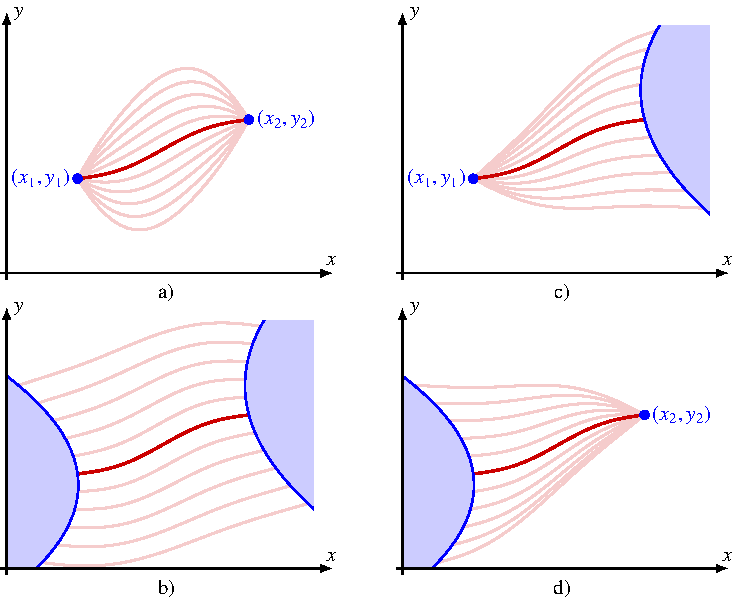
\includegraphics{chapters/020-variation/images/grundaufgaben.pdf}
\caption{Grundaufgaben der Variationsrechnung für eine Funktion $y(x)$.
a) Anfangspunkt-Endpunkt-Problem,
\index{Anfangspunkt-Endpunkt-Problem}%
b) Anfangskurve-Endkurve-Problem,
\index{Anfangskurve-Endkurve-Problem}%
c) Anfangspunkt-Endkurve-Problem,
\index{Anfangspunkt-Endkurve-Problem}%
d) Anfangspunkt-Endkurve-Problem
\index{Anfangspunkt-Endkurve-Problem}%
\label{buch:variation:problem:fig:grundaufgaben}}
\end{figure}

Das Brachistochronenproblem sucht eine Kurve, die zwei Punkte miteinander
verbindet.
Dies ist bekannt als das {\em Anfangspunkt-Endpunkt-Problem}.
\index{Anfangspunkt-Endpunkt-Problem}.
Andere Aufgabenstellungen sind jedoch auch denkbar.
Ein Schwimmer startet seine Flussüberquerung an einem Punkt
und will am anderen Ufer das Wasser wieder verlassen.
In welchem Punkt das geschieht, ist weniger wichtig.
In dieser Situation ist der Anfangspunkt vorgegeben, der Endpunkt ist
weniger eingeschränkt, er muss nur auf einer Kurve liegen.
Dies ist das {\em Anfangspunkt-Endkurve-Problem}.
Abbildung~\ref{buch:variation:problem:fig:grundaufgaben}
\index{Anfangspunkt-Endkurve-Problem}
zeigt alle möglichen Kombinationen.

Sobald bei der Lösung eines Problems mit gegebener Anfangs- oder Endkurve
die Punkte bekannt sind, in denen die Lösungskurve auf die Randkurven
trifft, ist das Problem auf ein Anfangspunkt-Endpunkt-Problem reduziert.
Es ist daher zunächst nötig, ein robustes Verfahren für diesen Grundfall
zu finden.
Die in Abschnitt~\ref{buch:variation:section:eulerlagrange}
abgeleitete Euler-Lagrange-Differentialgleichung behandelt diesen
Fall.
Sie ermöglicht, für jedes Paar von Punkten auf den Randkurven
eine Lösung zu finden.
Es sind dann weitere Bedingungen notwendig, welche die Anfangs- und
Endpunkte zu bestimmen gestatten.
In Kapitel~\ref{buch:chapter:nebenbedingungen} werden die sogenannten
Transversalitätsbedingungen hergeleitet, die vorschreiben, wie die
Lösungskurven auf die Randkurven treffen müssen.
Dadurch werden die Anfangs- und Endpunkte bestimmt.

Weitere denkbare Aufgabenstellungen könnten Kurven sein, deren Endpunkte
überhaupt nicht festgelegt sind oder Kurven, die einen Punkt enthalten
oder eine andere Art von Eigenschaft haben.
Kapitel~\ref{buch:chapter:nebenbedingungen} behandelt auch solche
Nebenbedingungen.


